

\section{Experimentation and Evaluation}
\label{sec:experiments}
\evalcomment{This retained Evaluation predates the active Unified BRCC method. Replace it with the registered matched experiments for calibration eligibility, exact weighted semantic coverage, coverage-preserving secondary refinement, shared-stacker utility, and logical cost. Until then, no result below supports a claim in the active paper.}

In this section, we first show the evaluation of experiments on four cybersecurity datasets.
Then, We present ablation studies of \Fname to investigate the robustness as well as the performance under different FL scenarios.

\subsection{Experimentation Setup}

The experiments are conducted on a machine installed Ubuntu 20.04 LTS with one CPU AMD Ryzen Threadripper 3960X and 96GB memory.
We use a client--server FL simulation environment comprising a client module and a server module, and the training process follows FedAvg~\cite{federated_learning}.

\subsubsection{Datasets}
We conduct experiments on the following datasets: a partition sampled from CIC-DDoS2019\cite{cicddos19} (DDoS2019), CICMalDroid2020\cite{maldroid} (MalDroid2020), CIC-Darknet2020\cite{darknet} (Darknet2020), and CIRA-CIC-DoHBrw-2020\cite{DoH} (DoHBrw2020).
The datasets DDoS2019, Darknet2020, and DoHBrw-2020 contain traffic packet statistic data, \eg flow rate and mean of packet size \etc of network for DDoS attack classification, darknet traffic, and DNS-over-HTTPS (DoH) traffic.
The Maldroid2020 is an Android malware classification dataset containing static and dynamic analysis patterns for 11,598 Android samples.
% All the datasets are timely and represent the newest cybersecurity data benchmark.

For the dataset DDoS2019, we select 3,355,966 samples as the training dataset and the remaining 1,127,526 samples as the test dataset.
Then, in order to prove that \Fname is able to detect the unknown attack as well, we keep the attack ``PORTMAP'' only in the test dataset which means such an attack is not included in the NIDS training process.
%To further prove that our method can detect an unseen attack, we leave the attack ``PORTMAP'' in the test dataset, \ie ``PORTMAP'' attack is not in the training data but exists in test data.
As for the rest three datasets, we randomly take $30\%$ data as test data. The details of the datasets are shown in \tablename~\ref{tab:datasets}.

\subsubsection{Data preprocessing: masking \& partition}
As mentioned in Section. \ref{sec:problem}, we adopt the following data masking for privacy protection:
\begin{packeditemize}
    \item Random feature data masking with $p=0.1$.
    \item Random label noise with $q=0.2$.
\end{packeditemize}

The training data are divided into 66 disjoint parts.
Each part represents data held by a client of the FL setting.
We show the class distribution of the DDoS2019 partition in Fig~\ref{fig:ddos_distribution}. Each client's data contain benign data and at most two different types of attack.

For other datasets, the client data are partitioned in a homogeneous way, \ie data of different classes are equally distributed, with the goal to investigate whether heterogeneous data partition would affect the performance.



\begin{figure}[htbp]
    \centering
    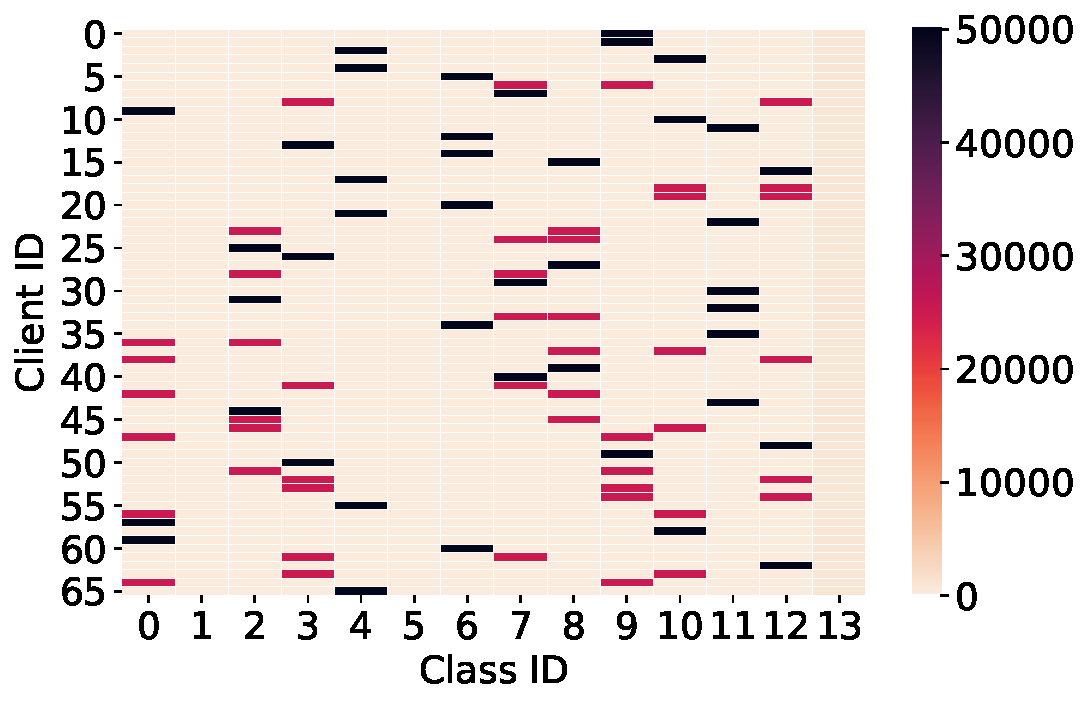
\includegraphics[width=0.85\linewidth]{figures/ddos_distribution.pdf}
    \caption{Class distribution of dataset DDoS2019.}
    \label{fig:ddos_distribution}
\end{figure}


\begin{table}[!ht]
\centering
\caption{Statistics of the four datasets.}
\label{tab:datasets}
\begin{tabular}{cccc}
\toprule
\textbf{Dataset}                           & \textbf{\# Features}  & \textbf{\# Class} & \textbf{\# Samples} \\ \hline
DDoS2019                               & 79                    & 14                & 4,483,492  \\ \hline
MalDroid2020                            & 470                   & 5                 & 11,598             \\ \hline
Darknet2020                            & 76                    & 11                & 141,483              \\ \hline
DoHBrw2020                       & 29                    & 4                 & 1,428,407                 \\
\bottomrule
\end{tabular}
\end{table}



\subsubsection{Baseline model reproduction}
We choose FedAvg~\cite{federated_learning} with MLP models of $3$, $5$, and $7$ layers as our baseline models. Each hidden layer of MLP has $64$ neurons, and the output layer is equal to the number of classes. We also compare our results with centralized training approaches including XGBoost\cite{xgboost} (noted as X) and
LightGBM\cite{lightgbm} (noted as L) which can be seen as the best performance achieved by GBDT if we gather client data to the server.

DP-GBDT~\cite{dpfedtree_ccs22} \dt{todo}


In our implementation, since MLP models are sensitive to the scale of data as well as infinity (Inf) and missing values (NaN), we first replace invalid values with $0$, then we preprocess the rest data in order to stabilize the training:

\begin{packeditemize}
    \item Logarithm operation. To reduce the order of magnitude of training data $\mathbf{X}$, for $i$-th column $\mathbf{X}[i]$, $\mathbf{X}[i]\leftarrow \log(\mathbf{X}[i]-\min(\mathbf{X}[i])+1)$, where $\min(\mathbf{X}[i])$ is minimum value of $\mathbf{X}[i]$.
    \item Standardization. For $i$-th column $\mathbf{X}[i]$, $\mathbf{X}[i]\leftarrow \frac{\mathbf{X}[i] - mean(\mathbf{X}[i])}{std(\mathbf{X}[i])}$, where $mean$ and $std$ stand for mean and standard deviation value of the column, respectively. Note that this preprocessing operation does not apply to binary feature.
\end{packeditemize}

To evaluate the performance of MLP, it is necessary to apply the same preprocessing for test data using the min, mean, and standard deviation values that are calculated for preprocessing training data.
Remark that computing min, mean, and standard deviation of each column is achievable under FL setting: it only needs to compute the sum, the squared sum as well as the number of samples of client data to compute a global value of mean and standard deviation.

We train each MLP model to achieve the highest accuracy score by gird search of hyperparameters: learning rate $lr\in\{0.1, 0.01\}$, maximum round of training for 1,000, 1,500 and 2,000, client batch size of each round 64, 128, and 256.
We test SGD and Adam\cite{adam} as optimizers.

We use raw data for GBDT models we used for experiments, \ie XGBoost and LightGBM, as they are not sensitive to the order of magnitude and data noise.
The most influential hyperparameters are been optimized through grid search: $n\_estimators$ ranges from 30 to 200 with step 10, $max\_depth$ from 4 to 10. As for LightGBM, $num\_leaves$ needs to be adjusted according to $max\_depth$, we set $num\_leaves = \lfloor \frac{2}{3}2^{max\_depth} \rfloor$.

\subsubsection{Metrics}
To evaluate the classification performance, we measure and compare the accuracy score, \ie the ratio of correctly classified samples in the test dataset.
Another important function of NIDS is the attack detection rate, \ie the ability to precisely distinguish malicious and benign data.
Here, we use the miss rate, \ie the ratio of attack data that are falsely classified as benign over all the benign predictions.
We also use the F1 score to evaluate the attack detection performance, as it pays equal attention to the precision and recalls in binary classification tasks.

\subsection{Comparison with baseline models}

We note ``Client GBDT+Server GBDT'' to clarify the model applied on clients and on the serve.
For example, ``X+L'' signifies that the client encoder model is XGBoost and the server model is LightGBM.
For this experiment, we set the budget of training data $B_t$ as the length of the dataset, and select all the encoders for encoder distribution of the second step.
In the ablation study, we will investigate the influence of our two heuristics on the performance in case the amount of clients becomes too large.

\evalcomment{Replace this comparison with the registered controls receiving the same frozen candidate pool, selection-calibration records, logical-byte budget, stacker-fit records, classifier capacity, and tuning allowance. Report methods that retrain base detectors separately because they assume different inputs.}


\subsubsection{Classification accuracy}\label{sec:classACC}

We report the accuracy scores in \tablename~\ref{tab:results}.
Bold numbers are the highest accuracy scores obtained on the datasets under the FL setting.
We can see that \Fname of architecture ``L+L'' achieves systematically higher accuracy against MLP models under FL settings.
The accuracy scores are comparable with the centralized training version of GBDT.
The results demonstrate the superiority over \acp{nn} for homogeneous as well as heterogeneous data partition, and that our NIDS is scalable for different tasks.

Remark that LightGBM model and \Fname with LightGBM achieve higher accuracy comparing with XGBoost model. The reason is that LightGBM is based on leaf-wise tree growth when constructing trees, which empowers \Fname with better data noise tolerance ability.
Another benefit of leaf-wise growth is the reduction of training complexity and model size.
Consequently, we use ``L+L'' as the default architecture of \Fname for further analysis. As for comparison, we choose 3-layer MLP  (fastest) and 7-layer MLP (most accurate) for \acp{nn}-based NIDS with FedAvg.

\subsubsection{Detection performance}

Since the dataset Darknet2020 contains only different types of darknet traffic instead of attack traffic, we choose the rest three datasets to examine the detection performance. We show the miss rates (left) and F1 scores (right) in \tablename~\ref{tab:detection}. The detection performance of \Fname is close to GBDT model (LightGBM) with centralized training (the ideal best performance) and obtains systematically better detection ability than FedAvg with MLP. Note that the miss rates of MLP with FedAvg on DDoS2019 are much higher, because there is little true benign data in the test dataset (only takes 0.28\%), and the predictions of MLP model contain many false-negative errors.


\begin{table}[!h]
\centering
\small
\caption{The miss rates and F1 scores for FedAvg with MLP,  LightGBM with centralized training and \Fname (L+L).}
\label{tab:detection}
\resizebox{0.95\columnwidth}{!}{
\begin{tabular}{cccc}
\toprule
\textbf{NIDS Model} & \textbf{DDoS2019} & \textbf{MalDroid2020} & \textbf{DoHBrw2020} \\ \hline
FedAvg 3-layer      & 93.24 \% / 12.65  & 15.38\% / 72.86       & 12.56\% / 92.27     \\ \hline
FedAvg 7-layer      & 93.31\% / 12.52   & 28.51\% / 68.04       & 5.86\% / 94.17      \\ \hline
LightGBM            & 4.42\% / 94.31    & 6.55\% / 90.84        & 1.00\% / 99.45      \\ \hline
\Fname (L+L)   & 4.40\% / 94.60    & 7.72\% / 88.59        & 0.71\% / 99.54      \\ \bottomrule
\end{tabular}
}
\end{table}

As for the unseen attack ``PORTMAP'' of DDoS2019 in the test data, both FedAvg (7-layer) locally trained GBDT and \Fname (L+L) can detect the attack with $100\%$ success rate, and classify the attack to ``NetBIOS'' with high confidence.
Since this category of attack (``PORTMAP'' attack) is not labeled and unknown to \Fname, \Fname classifies them all as the similar category ``NetBIOS''.
Thus, \Fname can effectively detect unknown attacks to generate anomaly alarms.



\begin{table*}[!ht]
\centering
\small
\caption{Accuracy scores of different FL models on four cybersecurity datasets.}
\label{tab:results}
\begin{tabular}{cccccc}
\toprule
\textbf{NIDS Model}                                                             & \textbf{Architecture} & \textbf{DDoS2019} & \textbf{MalDroid2020} & \textbf{Darknet2020} & \textbf{DoHBrw2020} \\ \hline
\multirow{3}{*}{\begin{tabular}[c]{@{}c@{}}\acp{nn} - MLP\\ FedAvg~\cite{federated_learning}\end{tabular}} & 3-layer        & 60.29             & 81.26                 & 55.71                & 75.85               \\ \cline{2-6}
& 5-layer        & 61.37             & 81.36                 & 55.58                & 76.92               \\ \cline{2-6}
 & 7-layer        & 61.74             & 80.68                 & 56.78                & 76.93               \\ \hline
% \multirow{2}{*}{\begin{tabular}[c]{@{}c@{}}GBDT\\ centralized training\end{tabular}}       & X              & 66.17            & 90.29                 & 87.48                & 79.80               \\ \cline{2-6}
%                                                                             & L              & 66.83             & 90.32                 & 87.56                & 80.75               \\ \hline
\multirow{4}{*}{\textbf{\Fname (Ours)}} & X+X & 66.34 & 89.45 & 85.24 & 78.87               \\ \cline{2-6}
 & L+X & 66.28 & 89.17 & 85.37 & 79.04 \\ \cline{2-6}
 & X+L & 65.76 & 88.90 & 85.78 & 79.20 \\ \cline{2-6}
 & L+L & \textbf{67.03} & \textbf{89.63} & \textbf{86.76} & \textbf{79.63} \\ \bottomrule
\end{tabular}
\end{table*}

\subsection{Result Analysis}
\subsubsection{Quality of feature extraction}
The goal of using encoders in \Fname is to remove noise and private information of raw data and extract feature representations, which can be seen as a method of data preprocessing.
To interpret the performance of our encoders considering the feature extraction, we choose DDoS2019 data as an example and use t-SNE~\cite{tsne} to visualize encoding data (\figurename~\ref{fig:visualize} (a)), as well as data preprocessed by logarithm operation (\figurename~\ref{fig:visualize} (b)) and followed standarization operation (\figurename~\ref{fig:visualize} (c)).

We observe that in the comparison with single logarithm operation, a followed standardization demonstrates better clustering ability for certain classes (\eg~Class 12, blue points), while it still cannot deal with other classes (\eg Class 10, green points) which indicates the weakness of handcrafted preprocessing methods.
As shown in \figurename~\ref{fig:visualize} (a), the representation of encoding data is less divergent, signifying that encoders outperform others in clustering characteristics for all classes.
Considering the data and label noise, most samples belonging to the same class are still successfully clustered.
This explains the superiority of \Fname over naive preprocessing techniques for \acp{nn}.

\begin{figure*}[htbp]

	    \centering
		\includegraphics[width=\linewidth]{figures/visualize.pdf}
		\caption{Visualization of encoding data (\textbf{left}) and preprocessed data by log (\textbf{middle}) and standarization (\textbf{right}).}
		\label{fig:visualize}

\end{figure*}

\subsubsection{Efficiency Analysis}
Here we use the DDoS2019 dataset as an example to evaluate the training overhead.
We report in \tablename~\ref{tab:training_overhead} average training overhead required by one client (second row) and the server (third row) for FedAvg using 3-layer MLP and 7-layer MLP and \Fname (architecture L+L).
We observe that the total overhead of \Fname is much lower than \acp{nn} when only using CPU for training.
The reduction is because of the small overhead on the client since the encoders are much smaller than the server classifier. Moreover, most importantly, they do not require updating parameters multiple times like \acp{nn} do which proves that \Fname is lightweight and easy to deploy on resource-constrained devices without accelerator like GPUs.
% \qiuhan{Total does not equal to the sum?}

\begin{table}[htbp]
\centering
\footnotesize
\caption{Training overhead of FedAvg (3-layer and 7-layer MLP) and \Fname (L+L) on DDoS2019 dataset.}
\label{tab:training_overhead}
\begin{tabular}{cccc}
\toprule
\textbf{Model} & \multicolumn{1}{l}{\textbf{3-layer MLP}} & \textbf{7-layer MLP} & \textbf{\Fname} \\ \hline
One Client   & 12.25s                           & 24.83s      & 0.22s             \\ \hline
Server   & 101.12s                          & 241.01s     & 201.26s           \\ \hline
Simulation Time   & 909.30s                           & 1879.78s    & 215.78s           \\ \bottomrule
\end{tabular}
\end{table}

% \noindent{\textbf{Communication Overhead.}}
We analyze the communication cost required by \acp{nn}-based NIDS and \Fname.
To quantify communication cost, we measure the transmission data size, \ie the data sent between server and clients during training.

For the NN-based NIDS model trained by FedAvg, the server sends model parameters to each client and received updated parameters from clients each round.
Therefore, the communication cost for uploading and downloading are equal, and the complexity is $O(KNR)$, where $R$ is the number of training rounds, and $K$ is the model size and $N$ is the number of participants.
In our experiment, we set $R=1000$ and $N=66$.
The model size refers to the weight and bias parameters of MLP, and $K$ equals $14286$ and $30926$ respectively for 3-layer and 7-layer MLPs ($79$ neurons for input layer, $14$ neurons for output layer, and $64$ neurons per hidden layer).

For \Fname, the uploading and downloading costs are different for the training is different from FedAvg. Specifically, each client uploads trained encoder and encoding data, which takes $O(KN + B_t\times (c_M M +1))$, where $K$ is encoder size, $B_t$ is predefined training data budget, and $c_M$ the average number of classes of encoder among $M$ selected encoders.
The last $1$ signifies label data.
The clients download $M$ selected encoders, which demands $O(KNM)$.
In our experiment, we take all the client data and all the encoders, thus $B_t=3355966$, $M=N=66$ and $c_M M =156$.
The largest encoder contains $3\times 60$ trees (3 classes and $n\_estimators$ 60) and each tree contains $10$ leaves, thus the encoder size $K$ is smaller than $10 \times 60 \times 3 = 1800$.

We summarize complexity and parameter number for uploading and downloading in \tablename~\ref{tab:communication_overhead}, and transmission data size when each parameter takes $8$ bytes in memory. We observe that FedAvg takes a larger flow quantity than \Fname. More importantly, the downloading data size is much bigger than that of \Fname, which further hinders training speed, since the downloading is generally slower than uploading and the clients need more time to download parameters.
As for \Fname, the clients only need to download selected encoders for accelerating the total training process.

\begin{table*}[htbp]
\centering
   \small
\caption{Communication overhead of FedAvg (3-layer and 7-layer MLP) and \Fname (L+L) on DDoS2019 dataset.}
\label{tab:communication_overhead}
\begin{tabular}{cccc}
\toprule
\textbf{NIDS Models}       & \textbf{3-layer MLP}                & \textbf{7-layer MLP}                  & \textbf{\Fname (L+L)} \\ \hline
Uploading Complexity          & \multicolumn{2}{c}{\multirow{2}{*}{$O(KNR)$}}                                & $O(KN  + B_t\times (c_M M+1))$    \\ \cline{1-1} \cline{4-4}
Downloading Complexity        & \multicolumn{2}{c}{}                                                       & $O(KNM)$                     \\ \hline
Uploading Parameters / Size   & \multirow{2}{*}{942876000 / 7.03GB} & \multirow{2}{*}{2041116000 / 15.21GB} & 526965862 / 3.92GB         \\ \cline{1-1} \cline{4-4}
Downloading Parameters / Size &                                     &                                       & 7840800 / 7.48MB           \\ \bottomrule
\end{tabular}
\end{table*}



% Note the class distribution is not private information that should be protected, because even for FedAvg, the server can easily infer it by checking the last layer

\evalcomment{The masking and Laplace-noise results below belong to the previous method and do not evaluate the active selector. Replace them with matched sensitivity studies for the eligibility threshold, semantic support threshold, budget fraction, calibration size, and secondary weights.}




\subsection{Ablation study}
We investigate the impact of parameters on the performance using DDoS2019 as an example.
We use LightGBM as the encoder and classifier for \Fname.
For comparison, we focus on 3-layer and 7-layer MLP as baseline models.
Unless otherwise specified, we use the same hyperparameters optimized by grid search as above.

\subsubsection{Accuracy score (ACC) of different data masking}

As mentioned in Section~\ref{sec:problem}, the clients generate random masking on the feature and label data before the training starts.
Another benefit is that the clients do not need to transmit the masked data to the server and further reduce communication overhead.
However, the masked data may contain critical features and decrease the model's performance.
Particularly, the masking on the feature data is more worth studying since it covers the majority of the data, \ie feature data.
Thus, we investigate the impact of feature data masking on the model.
\begin{figure}[htbp]
    \centering
    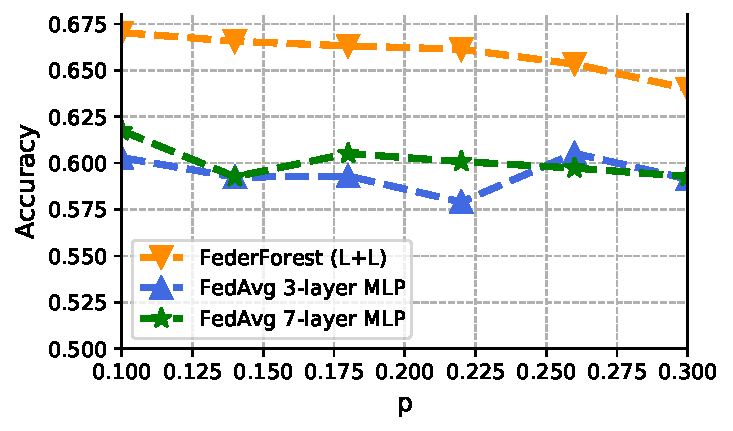
\includegraphics[width=0.95\linewidth]{figures/data_masking.pdf}
    \caption{ACC of \Fname and FedAvg for different data masking parameters $p$.}
    \label{fig:data_masking}
    % \vspace{2mm}
\end{figure}

The averaged ACC for different data masking parameters $p$ of \Fname (L+L) and FedAvg (3-layer MLP and 7-layer MLP) are shown in \figurename~\ref{fig:data_masking}.
Except for $p=0.26$, \Fname achieves systematically higher score.
We also notice that, comparing with \acp{nn}-based model, the performance of \Fname is more sensitive to the change of data masking under the same hyperparameters, as the accuracy score drops larger than 3-layer MLP and 7-layer MLP.
\subsubsection{Training Budget \& Encoder Selection}
\begin{figure}[htbp]
    \centering
    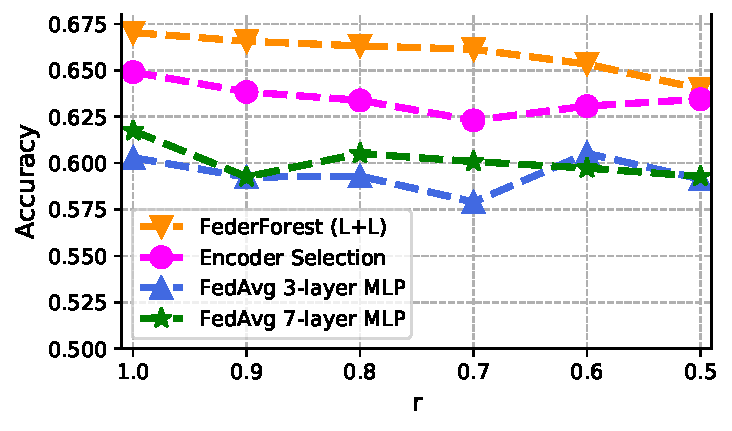
\includegraphics[width=0.95\linewidth]{figures/data_selection.pdf}
    \caption{ACC for different training budgets of ratio $r$.}
    \label{fig:data_selection}
    % \vspace{2mm}
\end{figure}

In \figurename~\ref{fig:data_selection}, we present the accuracy for different training budget ratios $r =\frac{B_t}{n}$, where $n$ is the total amount of training data. As illustrated in the figure, the training budget has little influence on the ACC achieved by \Fname, \Fname with encoder selection and FedAvg, as the data are drawn from the same distribution.

After selected encoders, the size of encoding data is also reduced, therefore it is necessary to readjust the hyperparameters of the global classifier using grid search. Notice that the introduced encoder selection slightly decreases the accuracy score, because there are fewer features in the encoding data used for training the global classifier. However, the encoder selection reduces the communication overhead. In our experiments, at most 8 encoders are selected while there are 66 in total, which means the communication overhead of transferring encoding data is reduced at least 80\%.

\subsubsection{\red{Laplace-Noise Parameter}}

\begin{figure}[htbp]
    \centering
    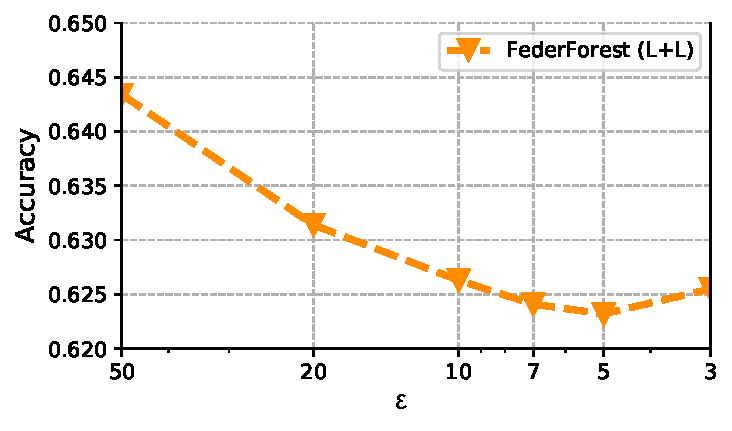
\includegraphics[width=0.95\linewidth]{figures/dp_epsilon.pdf}
    \caption{\red{ACC for different per-block Laplace-noise parameters $\epsilon$.}}
    \label{fig:dp_epsilon}
    % \vspace{2mm}
\end{figure}

\red{We investigate how the per-encoder-block parameter $\epsilon$ affects accuracy. Specifically, Figure~\ref{fig:dp_epsilon} reports the accuracy of \Fname at $\epsilon\in\{50,20,10,7,5,3\}$. As $\epsilon$ decreases, the added Laplace noise increases and accuracy falls. Because we do not analyze the full protocol, $\epsilon$ is only the noise parameter used here and not an end-to-end privacy budget for \Fname.}


\subsection{Machine Unlearning}

The right to be forgotten attracts increasing attention and is protected by legislations such as the General Data Protection Regulation (GDPR)~\cite{gdpr} in Europe.
Bourtoule~\etal have introduced machine unlearning \cite{unlearning} which aims to erase the effect of data to be unlearned from a trained model.
They have also proposed SISA, a training framework that allows data to be unlearned from the model with a minimal cost.
Specifically, SISA partitions the training dataset into small parts called shards, and train one constituent model for each shard.
In this way, when some data need to be unlearned, only the model of the shard containing the data has to be retrained from the last checkpoint where the data is not introduced into the training process.

For the machine unlearning, \Fname is designed to be similar to the SISA by regarding client data as the shards.
If some client wants to be unlearned, it only needs to delete the corresponding encoding data and retrain the server classifier.
For the client who wants to be unlearned but whose encoder has been spread to other clients during training, the server has to select another available encoder to encode client data.
Nevertheless, the major cost is still retraining the server classifier. Consequently,
\Fname allows participants to freely unlearn data without exerting much influence on the server.





% \begin{figure*}[!ht]

% 	    \centering
% 		\includegraphics[width=0.32\textwidth]{figures/logminusmin.pdf}
% 		\includegraphics[width=0.32\textwidth]{figures/logminusmin_normalization.pdf}
% 		\includegraphics[width=0.32\textwidth]{figures/encoded.pdf}
% 		\caption{(Best viewed in color) Visualization of preprocessed data by log(\textbf{left}), standarization (\textbf{middle}) and GBDT encoded data (\textbf{right}) by t-SNE}
% 		\label{fig:visualize}

% \end{figure*}
